\subsection{BÀI TẬP TRẮC NGHIỆM}

\Opensolutionfile{ans}[ans/1H4.B1]
\setcounter{ex}{0}
\begin{ex}%[1H2Y1-1]
	Cho tứ giác $ABCD$. Có thể xác định được bao nhiêu mặt phẳng chứa tất cả các đỉnh của tứ giác $ABCD$?
	\choice
	{\True $1 $}
	{$3 $}
	{$0 $}
	{$2 $}
	\loigiai{
		$4$ điểm $A,B,C,D$ tạo thành $1$ tứ giác, khi đó $4$ điểm $A,B,C,D$ đã đồng phẳng và tạo thành $1$ mặt phẳng duy nhất là mặt phẳng $\left(ABCD\right)$.}
\end{ex}

\begin{ex}%[1H2Y1-1]%
	Hình chóp tam giác có số cạnh là
	\choice
	{\True $ 6 $}
	{$ 4 $}
	{$ 5 $}
	{$ 3 $}
	\loigiai{
		\immini{Xét hình chóp tam giác $ S.ABC $ có các cạnh là $ SA $, $ SB $, $ SC $, $ AB $, $ BC $ và $ CA $. Vậy hình chóp có số cạnh là $ 6 $.}
		{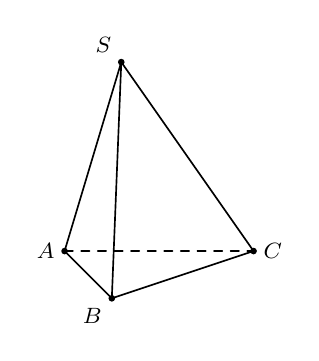
\begin{tikzpicture}[line join=round,line cap=round,line width=.6pt,font=\footnotesize,scale=0.6]
				\coordinate[label=left:$A$] (A) at (0,0);
				\coordinate[label=below left:$B$] (B) at (1,-1);
				\coordinate[label=right:$C$] (C) at (4,0);
				\coordinate[label=above left:$S$] (S) at (1.2,4);
				\draw (A)--(B)--(C)--(S)--cycle (S)--(B);
				\draw[dashed] (A)--(C);
				\fill (A)circle(2pt) (B)circle(2pt) (C)circle(2pt) (S)circle(2pt);
			\end{tikzpicture}
		}
	}
\end{ex}

\begin{ex}%[1H2B1]
	Hình chóp lục giác có bao nhiêu mặt?
	\choice
	{$10$}
	{$6$}
	{$8$}
	{\True $7$}
	\loigiai{
		Hình chóp có $7$ mặt trong đó có $6$ mặt bên và $1$ mặt đáy.}
\end{ex}


\begin{ex}%[1H2Y1-1]
	Các yếu tố nào sau đây xác định một mặt phẳng duy nhất?
	\choice
	{Một điểm và một đường thẳng}
	{\True Hai đường thẳng cắt nhau}
	{Bốn điểm phân biệt}
	{Ba điểm phân biệt}
	\loigiai{
		\begin{itemize}
			\item Mệnh đề \lq\lq Ba điểm phân biệt\rq\rq\  sai. Trong trường hợp $3$ điểm phân biệt thẳng hàng thì sẽ có vô số mặt phẳng chứa $3 $ điểm thẳng hàng đã cho.
			\item Mệnh đề \lq\lq Một điểm và một đường thẳng\rq\rq\ sai. Trong trường hợp điểm thuộc đường thẳng đã cho, khi đó ta chỉ có $1$ đường thẳng, có vô số mặt phẳng đi qua đường thẳng đó.
			\item  Mệnh đề \lq\lq Bốn điểm phân biệt\rq\rq\ sai. Trong trường hợp $4$ điểm phân biệt thẳng hàng thì có vô số mặt phẳng đi qua $4$ điểm đó hoặc trong trường hợp $4$ điểm mặt phẳng không đồng phẳng thì sẽ không tạo được mặt phẳng nào đi qua cả $4$ điểm.
	\end{itemize}}
\end{ex}

\begin{ex}%[1H2Y1]
	Khẳng định nào sau đây là \textbf{sai}?
	\choice
	{Nếu hai mặt phẳng phân biệt có một điểm chung thì chúng có một đường thẳng chung duy nhất}
	{Nếu hai mặt phẳng có một điểm chung thì chúng có vô số điểm chung khác nữa}
	{Nếu ba điểm phân biệt cùng thuộc hai mặt phẳng phân biệt thì chúng thẳng hàng}
	{\True  Nếu hai mặt phẳng có một điểm chung thì chúng có một đường thẳng chung duy nhất}
	\loigiai{
		Hai mặt phẳng có một điểm chung thì có thể trùng nhau, khi đó chúng có vô số đường thẳng chung.
	}
\end{ex}

\begin{ex}%[1H2Y1-1]
	Cho $5$ điểm $A,B,C,D,E$ trong đó không có $4$ điểm nào đồng phẳng. Hỏi có bao nhiêu mặt phẳng tạo bởi $3$ trong $5$ điểm đã cho?
	\choice
	{\True $10 $}
	{$14 $}
	{$12 $}
	{$8 $}
	\loigiai{
		Với $3$ điểm phân biệt không thẳng hàng, ta luôn tạo được $1$ mặt phẳng xác định.
		Ta có $\mathrm{C}_5^3$ cách chọn $3$ điểm trong $5$ điểm đã cho để tạo được $1$ mặt phẳng xác định. Vậy số mặt phẳng tạo được là $10$.}
\end{ex}

\begin{ex}%[1H2Y1-1]
	Trong các khẳng định sau, khẳng định nào đúng?
	\choice
	{Qua $3$ điểm phân biệt bất kì có duy nhất một mặt phẳng}
	{Qua $4$ điểm phân biệt bất kì có duy nhất một mặt phẳng}
	{Qua $2$ điểm phân biệt có duy nhất một mặt phẳng}
	{\True Qua $3$ điểm không thẳng hàng có duy nhất một mặt phẳng}
	\loigiai{
		\begin{itemize}
			\item Mệnh đề \lq\lq Qua $2$ điểm phân biệt có duy nhất một mặt phẳng\rq\rq\ sai. Vì qua $2 $ điểm phân biệt, tạo được $1$ đường thẳng, khi đó chưa đủ điều kiện để lập một mặt phẳng xác định. Có vô số mặt phẳng đi qua $2$ điểm đã cho.
			\item Mệnh đề \lq\lq Qua $3$ điểm phân biệt bất kì có duy nhất một mặt phẳng\rq\rq\ sai. Vì trong trường hợp $3$ điểm phân biệt thẳng hàng thì chỉ tạo được đường thẳng, khi đó có vô số mặt phẳng đi qua $3$ điểm phân biệt thẳng hàng.
			\item Mệnh đề \lq\lq Qua $4$ điểm phân biệt bất kì có duy nhất một mặt phẳng\rq\rq\ sai. Vì trong trường hợp $4$ điểm phân biệt thẳng hàng thì có vô số mặt phẳng đi qua $4$ điểm đó hoặc trong trường hợp $4$ điểm mặt phẳng không đồng phẳng thì sẽ tạo không tạo được mặt phẳng nào đi qua cả $4$ điểm.
	\end{itemize}}
\end{ex}

\begin{ex}%[Nguyễn Phúc Đức]%[1H2B1]
	Cho các hình vẽ sau: \\
	\begin{tabular}{cccc}
		\begin{tikzpicture}[scale=0.6,line width=1pt,line cap=round,line join=round,>=triangle 45,x=1.0cm,y=1.0cm]
			\clip(-3.48,0.6) rectangle (2.4,5.4);
			\draw (-1,5)-- (-3,2);
			\draw (-1,5)-- (0,1);
			\draw (-1,5)-- (2,2);
			\draw (-3,2)-- (0,1);
			\draw (0,1)-- (2,2);
			\draw [dash pattern=on 2pt off 2pt] (-3,2)-- (2,2);
			\fill [color=black] (-1,5) circle (1.5pt);
			\draw[color=black] (-0.8,5.2) node {$A$};
			\fill [color=black] (-3,2) circle (1.5pt);
			\draw[color=black] (-3.1,2.3) node {$B$};
			\fill [color=black] (0,1) circle (1.5pt);
			\draw[color=black] (-0.3,0.8) node {$C$};
			\fill [color=black] (2,2) circle (1.5pt);
			\draw[color=black] (2.2,2.3) node {$D$};
		\end{tikzpicture} & \begin{tikzpicture}[scale=0.6,line width=1pt,line cap=round,line join=round,>=triangle 45,x=1.0cm,y=1.0cm]
			\clip(-3.52,0.46) rectangle (2.56,5.48);
			\draw (-1,5)-- (-3,1);
			\draw (-1,5)-- (0,2);
			\draw (-1,5)-- (2,1);
			\draw (-3,1)-- (0,2);
			\draw (0,2)-- (2,1);
			\draw (-3,1)-- (2,1);
			\fill [color=black] (-1,5) circle (1.5pt);
			\draw[color=black] (-1.3,5.2) node {$A$};
			\fill [color=black] (-3,1) circle (1.5pt);
			\draw[color=black] (-3.14,1.26) node {$B$};
			\fill [color=black] (0,2) circle (1.5pt);
			\draw[color=black] (-0.04,1.6) node {$C$};
			\fill [color=black] (2,1) circle (1.5pt);
			\draw[color=black] (2.16,1.28) node {$D$};
		\end{tikzpicture} & \begin{tikzpicture}[scale=0.6,line width=1pt,line cap=round,line join=round,>=triangle 45,x=1.0cm,y=1.0cm]
			\clip(-3.42,0.58) rectangle (2.56,5.4);
			\draw (-1,5)-- (-3,1);
			\draw [dash pattern=on 2pt off 2pt] (-1,5)-- (0,2);
			\draw (-1,5)-- (2,1);
			\draw [dash pattern=on 2pt off 2pt] (-3,1)-- (0,2);
			\draw [dash pattern=on 2pt off 2pt] (0,2)-- (2,1);
			\draw (-3,1)-- (2,1);
			\fill [color=black] (-1,5) circle (1.5pt);
			\draw[color=black] (-1.3,5.2) node {$A$};
			\fill [color=black] (-3,1) circle (1.5pt);
			\draw[color=black] (-3.14,1.26) node {$B$};
			\fill [color=black] (0,2) circle (1.5pt);
			\draw[color=black] (-0.04,1.6) node {$C$};
			\fill [color=black] (2,1) circle (1.5pt);
			\draw[color=black] (2.16,1.28) node {$D$};
		\end{tikzpicture}& \begin{tikzpicture}[scale=0.6,line width=1pt,line cap=round,line join=round,>=triangle 45,x=1.0cm,y=1.0cm]
			\clip(-3.48,0.6) rectangle (2.4,5.4);
			\draw (-1,5)-- (-3,2);
			\draw (-1,5)-- (0,1);
			\draw (-1,5)-- (2,2);
			\draw (-3,2)-- (0,1);
			\draw (0,1)-- (2,2);
			\draw (-3,2)-- (2,2);
			\fill [color=black] (-1,5) circle (1.5pt);
			\draw[color=black] (-0.8,5.2) node {$A$};
			\fill [color=black] (-3,2) circle (1.5pt);
			\draw[color=black] (-3.1,2.3) node {$B$};
			\fill [color=black] (0,1) circle (1.5pt);
			\draw[color=black] (-0.3,0.8) node {$C$};
			\fill [color=black] (2,2) circle (1.5pt);
			\draw[color=black] (2.2,2.3) node {$D$};
		\end{tikzpicture} \\ 
		Hình $(1)$& Hình $(2)$ & Hình $(3)$ & Hình $(4)$
	\end{tabular} \\
	Trong các hình trên, những hình nào biểu diễn cho tứ diện?
	\choice{Hình (1) và hình (2)}
	{\True Hình (1), hình (2) và hình (3)}
	{Hình (1) và hình (3)}
	{Hình (1), hình (3) và hình (4)}
\end{ex}

\begin{ex}%[1H2B1-2]
\immini[thm]{Cho tứ diện $ABCD$. Gọi $M, N$ lần lượt là trung điểm của $AC,CD$. Giao tuyến của hai mặt phẳng $\left(MBD\right)$ và $\left(ABN\right)$ là
	\choice
	{\True đường thẳng $BG$ ($G$ là trọng tâm tam giác $ACD$)}
	{đường thẳng $AH$ ($H$ là trực tâm tam giác $ACD$)}
	{đường thẳng $MN $}
	{đường thẳng $AM $}
}{
	\begin{tikzpicture}[scale=0.6, line join=round, line cap=round]
	\tkzDefPoints{0/0/B,1.5/-1.8/C,4/0/D, 2/3/A}
	\tkzDefMidPoint(A,C)\tkzGetPoint{M}
	\tkzDefMidPoint(D,C)\tkzGetPoint{N}
	\tkzDrawPolygon(A,B,C,D)
	\tkzDrawSegments(A,C B,M D,M A,N)
	\tkzDrawSegments[dashed](B,D B,N)
	\tkzDrawPoints[fill=black](M,A,B,C,D,N)
	\tkzLabelPoints[above,font=\footnotesize](A)
	\tkzLabelPoints[below,font=\footnotesize](C,N)
	\tkzLabelPoints[left,font=\footnotesize](B)
	\tkzLabelPoints[right,font=\footnotesize](D)
	\tkzLabelPoints[above left,font=\footnotesize](M)
	\end{tikzpicture}}
	\loigiai{
		\immini{
			\begin{itemize}
				\item $B$ là điểm chung thứ nhất giữa hai mặt phẳng $\left(MBD\right)$ và $\left(ABN\right) $.
				\item Vì $M,N$ lần lượt là trung điểm của $AC,CD$ nên suy ra $AN,DM$ là hai trung tuyến của tam giác $ACD. $\\
				Gọi $G=AN\cap DM$
				$\Rightarrow \left\{\begin{aligned}& G\in AN\subset \left(ABN\right)\Rightarrow G\in \left(ABN\right) \\
				& G\in DM\subset \left(MBD\right)\Rightarrow G\in \left(MBD\right)
				\end{aligned}\right.$\\
				$\Rightarrow G$ là điểm chung thứ hai giữa hai mặt phẳng $\left( {MBD} \right)$ và $\left( {ABN} \right).$
			\end{itemize}
			Vậy $\left(ABN\right)\cap \left(MBD\right)=BG $.
		}
		{
			\begin{tikzpicture}[scale=1, line join=round, line cap=round]
			\tkzDefPoints{0/0/B,1.5/-1.8/C,4/0/D, 2/3/A}
			\tkzDefMidPoint(A,C)\tkzGetPoint{M}
			\tkzDefMidPoint(D,C)\tkzGetPoint{N}
			\tkzCentroid(D,A,C)\tkzGetPoint{G}
			\tkzDrawPolygon(A,B,C,D)
			\tkzDrawSegments(A,C B,M D,M A,N)
			\tkzDrawSegments[dashed](B,D B,G B,N)
			\tkzDrawPoints[fill=black](M,A,B,C,D,N,G)
			\tkzLabelPoints[above](A)
			\tkzLabelPoints[below](C,N)
			\tkzLabelPoints[left](B)
			\tkzLabelPoints[right](D)
			\tkzLabelPoints[above right](M,G)
			\end{tikzpicture}
		}
	}
\end{ex}

\begin{ex}%[1H2B1-2]
	\immini[thm]{Cho $4$ điểm không đồng phẳng $A,B,C,D$.  Gọi $I,K$ lần lượt là trung điểm của $AD$ và $BC$. Giao tuyến của $\left(IBC\right)$ và $\left(KAD\right)$ là
	\choice
	{\True $IK$}
	{$DK $}
	{$AK $}
	{$BC$}}{

\begin{tikzpicture}[scale=0.7, font=\footnotesize,>=stealth]
	\path
	%	Vẽ mp
	(0,0) coordinate (B)
	(5,0) coordinate (C)
	(1.5,-1.5) coordinate (D)
	(1,3.2) coordinate (A)
	($(A)!0.5!(D)$)coordinate (I)
	($(C)!0.5!(B)$)coordinate (K)
	;
	\draw (B)--(A)--(D)--(C)--(A) (B)--(D);
	\draw[dashed] (B)--(C);
	\foreach \x/\g in {B/180,A/90,C/0,D/-90,I/180,K/30}\draw[fill=black] (\x) circle (.05) +(\g:.5)node{\footnotesize$\x$};
\end{tikzpicture}}
	\loigiai{
		\immini{
			Điểm $K$ là trung điểm của $BC$ suy ra $K\in \left(IBC\right)\Rightarrow IK\subset \left(IBC\right) $.\\
			Điểm $I$ là trung điểm của $AD$ suy ra $I\in \left(KAD\right)\Rightarrow IK\subset \left(KAD\right) $.\\
			Vậy giao tuyến của hai mặt phẳng $\left(IBC\right)$ và $\left(KAD\right)$ là $IK$.
		}
		{
			\begin{tikzpicture}[scale=0.7, line join=round, line cap=round]
			\tkzDefPoints{0/0/B,1.5/-1.8/C,4/0/D, 2/2.5/A}
			\tkzDefMidPoint(C,B)\tkzGetPoint{K}
			\tkzDefMidPoint(A,D)\tkzGetPoint{I}
			\tkzDrawPolygon(A,B,C,D)
			\tkzDrawSegments(A,K C,I)
			\tkzDrawSegments[dashed](B,D B,I K,I K,D)
			\tkzDrawPoints[fill=black](K,A,B,C,D,I)
			\tkzLabelPoints[above](A)
			\tkzLabelPoints[above right](I)
			\tkzLabelPoints[below](C)
			\tkzLabelPoints[below left](K)
			\tkzLabelPoints[left](B)
			\tkzLabelPoints[right](D)
			\end{tikzpicture}
		}
	}
\end{ex}

\begin{ex}%[1H2B1-2]
	\immini[thm]{Cho tứ diện $ABCD$. Gọi $G$ là trọng tâm của tam giác $BCD$. Giao tuyến của mặt phẳng $\left(ACD\right)$ và $\left(GAB\right)$ là
	\choice
	{$AH$ ($H$ là hình chiếu của $B$ trên $CD) $}
	{$AM$ ($M$ là trung điểm của $AB) $}
	{$AK$ ($K$ là hình chiếu của $C$ trên $BD) $}
	{\True $AN$ ($N$ là trung điểm của $CD) $}
}{
	\begin{tikzpicture}[scale=0.7, line join=round, line cap=round]
	\tkzDefPoints{0/0/B,0.5/-1.5/C,4/0/D, 1.5/3/A}
	\tkzCentroid(D,B,C)\tkzGetPoint{G}
	\tkzDrawPolygon(A,B,C,D)
	\tkzDrawSegments(A,C)
	\tkzDrawSegments[dashed](B,D A,G B,G)
	\tkzDrawPoints[fill=black](G,A,B,C,D)
	\tkzLabelPoints[above](A)
	\tkzLabelPoints[below](C,G)
	\tkzLabelPoints[left](B)
	\tkzLabelPoints[right](D)
	\end{tikzpicture}}
	\loigiai{
		\immini{
			\begin{itemize}
				\item $A$ là điểm chung thứ nhất giữa hai mặt phẳng $\left(ACD\right)$ và $\left(GAB\right) $.
				\item Ta có $BG\cap CD=N$\\
				$ \Rightarrow \left\{\begin{aligned}& N\in BG\subset \left(ABG\right)\Rightarrow N\in \left(ABG\right) \\
				& N\in CD\subset \left(ACD\right)\Rightarrow N\in \left(ACD\right).
				\end{aligned}\right.$\\
				$\Rightarrow N$ là điểm chung thứ hai giữa hai mặt phẳng $\left(ACD\right)$ và $\left(GAB\right) $.
			\end{itemize}
			Vậy $\left( {ABG} \right) \cap \left( {ACD} \right) = AN.$
		}
		{
			\begin{tikzpicture}[scale=0.8, line join=round, line cap=round]
			\tkzDefPoints{0/0/B,0.5/-1.5/C,4/0/D, 1.5/3/A}
			\tkzDefMidPoint(D,C)\tkzGetPoint{N}
			\tkzCentroid(D,B,C)\tkzGetPoint{G}
			\tkzDrawPolygon(A,B,C,D)
			\tkzDrawSegments(A,C A,N)
			\tkzDrawSegments[dashed](B,D A,G B,N)
			\tkzDrawPoints[fill=black](G,A,B,C,D,N)
			\tkzLabelPoints[above](A)
			\tkzLabelPoints[below](C,G)
			\tkzLabelPoints[left](B)
			\tkzLabelPoints[right](D)
			\end{tikzpicture}
		}
	}
\end{ex}

\begin{ex}%[1H2B1-2]
\immini[thm]{Cho hình chóp $S.ABCD$ có đáy là hình thang $ABCD\left(AD\parallel BC\right) $. Gọi $M$ là trung điểm $CD $. Giao tuyến của hai mặt phẳng $\left(MSB\right)$ và $\left(SAC\right)$ là
	\choice
	{$SJ$ ($J$ là giao điểm của $AM$ và $BD$)}
	{\True $SI$ ($I$ là giao điểm của $AC$ và $BM$)}
	{$SO$ ($O$ là giao điểm của $AC$ và $BD$)}
	{$SP$ ($P$ là giao điểm của $AB$ và $CD$)}
}{
	\begin{tikzpicture}[scale=0.8, line join=round, line cap=round]
	\tkzDefPoints{0/0/A,0.5/-1.5/B,3/-1.5/C,4/0/D, 1/2/S}
	\tkzDefMidPoint(C,D)\tkzGetPoint{M}
	\tkzDrawPolygon(S,A,B,C,D)
	\tkzDrawSegments(S,C S,B S,M)
	\tkzDrawSegments[dashed](A,D A,C B,M)
	\tkzDrawPoints[fill=black](M,A,B,C,D,S)
	\tkzLabelPoints[above](S)
	\tkzLabelPoints[below](B,C)
	\tkzLabelPoints[left](A)
	\tkzLabelPoints[right](D,M)
	\end{tikzpicture}}
	\loigiai{
		\immini{
			\begin{itemize}
				\item  $S$ là điểm chung thứ nhất giữa hai mặt phẳng $\left(MSB\right)$ và $\left(SAC\right) $.\\
				\item  Ta có $\left\{\begin{aligned}& I\in BM\subset \left(SBM\right)\Rightarrow I\in \left(SBM\right) \\
				& I\in \left(AC\right)\in \left(SAC\right)\Rightarrow I\in \left(SAC\right)
				\end{aligned}\right.$\\
				$\Rightarrow I$ là điểm chung thứ hai giữa hai mặt phẳng $\left(SAC \right)$ và $\left(SAC\right).$
			\end{itemize}
			Vậy $\left(MSB\right)\cap \left(SAC\right)=SI $.
		}
		{
			\begin{tikzpicture}[scale=1, line join=round, line cap=round]
			\tkzDefPoints{0/0/A,0.5/-1.5/B,3/-1.5/C,4/0/D, 1/3/S}
			\tkzDefMidPoint(C,D)\tkzGetPoint{M}
			\tkzInterLL(A,C)(B,M)\tkzGetPoint{I}
			\tkzDrawPolygon(S,A,B,C,D)
			\tkzDrawSegments(S,C S,B S,M)
			\tkzDrawSegments[dashed](S,I A,D A,C B,M)
			\tkzDrawPoints[fill=black](M,A,B,C,D,I,S)
			\tkzLabelPoints[above](S)
			\tkzLabelPoints[above right](I)
			\tkzLabelPoints[below](B,C)
			\tkzLabelPoints[left](A)
			\tkzLabelPoints[right](D,M)
			\end{tikzpicture}
		}
	}
\end{ex}

\begin{ex}%[1H2B1-2]
	Cho hình chóp $S.ABCD$ có đáy là hình thang $ABCD\left(AB\parallel CD\right) $. Khẳng định nào sau đây \textbf{sai}?
	\choice
	{Hình chóp $S.ABCD$ có $4$ mặt bên}
	{Giao tuyến của hai mặt phẳng $\left(SAC\right)$ và $\left(SBD\right)$ là $SO$ ($O$ là giao điểm của $AC$ và $BD) $}
	{\True Giao tuyến của hai mặt phẳng $\left(SAB\right)$ và $\left(SAD\right)$ là đường trung bình của $ABCD$
	}
	{Giao tuyến của hai mặt phẳng $\left(SAD\right)$ và $\left(SBC\right)$ là $SI$ ($I$ là giao điểm của $AD$ và $BC) $}
	\loigiai{
		\immini{
			\begin{itemize}
				\item Hình chóp $S.ABCD$ có 4 mặt bên: $\left(SAB\right),\left(SBC\right),\left(SCD\right),\left(SAD\right) $.
				\item là điểm chung thứ nhất của hai mặt phẳng $\left(SAC\right)$ và $\left(SBD\right) $.
				$\left\{\begin{aligned}& O\in AC\subset \left(SAC\right)\Rightarrow O\in \left(SAC\right) \\
				& O\in BD\subset \left(SBD\right)\Rightarrow O\in \left(SBD\right)
				\end{aligned}\right.\Rightarrow O$ là điểm chung thứ hai của hai mặt phẳng $\left(SAC\right)$ và $\left(SBD\right).$\\
				$\Rightarrow \left(SAC\right)\cap \left(SBD\right)=SO $.
				\item Tương tự, ta có $\left(SAD\right)\cap \left(SBC\right)=SI $.
				\item $\left(SAB\right)\cap \left(SAD\right)=SA$ mà $SA$ không phải là đường trung bình của hình thang $ABCD $.
			\end{itemize}
			Vậy \lq\lq Giao tuyến của hai mặt phẳng $\left(SAB\right)$ và $\left(SAD\right)$ là đường trung bình của $ABCD$\rq\rq\ là mệnh đề sai.
		}
		{
			\begin{tikzpicture}[scale=1, line join=round, line cap=round]
			\tkzDefPoints{0/0/A,0.5/-1.5/D,4/0/B,2.4/-1.5/C, 1.5/3/S}
			\tkzInterLL(A,C)(B,D)\tkzGetPoint{O}
			\tkzInterLL(A,D)(B,C)\tkzGetPoint{I}
			\tkzDrawPolygon(S,A,I,B)
			\tkzDrawSegments(S,D S,C S,I)
			\tkzDrawSegments[dashed](S,O A,B D,C A,C B,D)
			\tkzDrawPoints[fill=black](S,A,B,C,D,O,I)
			\tkzLabelPoints[above](S)
			\tkzLabelPoints[below](O,I)
			\tkzLabelPoints[left](A,D)
			\tkzLabelPoints[right](C,B)
			\end{tikzpicture}
		}
	}
\end{ex}

\begin{ex}%[1H2B1-2]
\immini[thm]{Cho hình chóp $S.ABCD$ có đáy $ABCD$ là hình bình hành. Gọi $M, N$ lần lượt là trung điểm $AD$ và $BC$. Giao tuyến của hai mặt phẳng $\left(SMN\right)$ và $\left(SAC\right)$ là
	\choice
	{$SG$ ($G$ là trung điểm $AB$)}
	{$SD$}
	{\True $SO$ ($O$ là tâm hình bình hành $ABCD$)}
	{$SF$ ($F$ là trung điểm $CD$)}
}{
	\begin{tikzpicture}[scale=0.6, line join=round, line cap=round]
	\tkzDefPoints{0/0/A,-1.5/-1.8/B,4/0/D, 0.2/3/S}
	\coordinate (C) at ($(B)+(D)-(A)$);
	\tkzDefMidPoint(A,D)\tkzGetPoint{M}
	\tkzDefMidPoint(B,C)\tkzGetPoint{N}
	\tkzDrawPolygon(S,B,C,D)
	\tkzDrawSegments(S,C S,D S,N)
	\tkzDrawSegments[dashed](S,A A,B A,C M,N A,D S,M)
	\tkzDrawPoints[fill=black](M,A,B,C,D,N,S)
	\tkzLabelPoints[above](S)
	\tkzLabelPoints[above right](M)
	\tkzLabelPoints[below](B,C,N)
	\tkzLabelPoints[left](A)
	\tkzLabelPoints[right](D)
	\end{tikzpicture}}
	\loigiai{
		\immini{
			\begin{itemize}
				\item $S$ là điểm chung thứ nhất giữa hai mặt phẳng $\left(SMN\right)$ và $\left(SAC\right) $.
				\item Gọi $O=AC\cap BD$ là tâm của hình hình hành.
			\end{itemize}
			Trong mặt phẳng $\left(ABCD\right)$, gọi $T=AC\cap MN$\\
			$\Rightarrow \left\{\begin{aligned}& O\in AC\subset \left(SAC\right)\Rightarrow O\in \left(SAC\right) \\
			& O\in MN\subset \left(SMN\right)\Rightarrow O\in \left(SMN\right)
			\end{aligned}\right.$\\
			$\Rightarrow O$ là điểm chung thứ hai giữa hai mặt phẳng $\left(SMN\right)$ và $\left( {SAC} \right).$\\
			Vậy $\left(SMN\right)\cap \left(SAC\right)=SO $.
		}
		{
			\begin{tikzpicture}[scale=1, line join=round, line cap=round]
			\tkzDefPoints{0/0/A,-1.5/-1.8/B,4/0/D, 0.2/3/S}
			\coordinate (C) at ($(B)+(D)-(A)$);
			\tkzDefMidPoint(A,D)\tkzGetPoint{M}
			\tkzDefMidPoint(B,C)\tkzGetPoint{N}
			\tkzInterLL(A,C)(M,N)\tkzGetPoint{O}
			\tkzDrawPolygon(S,B,C,D)
			\tkzDrawSegments(S,C S,D S,N)
			\tkzDrawSegments[dashed](S,A A,B A,C M,N A,D S,O S,M)
			\tkzDrawPoints[fill=black](M,A,B,C,D,N,O,S)
			\tkzLabelPoints[above](S)
			\tkzLabelPoints[above right](M)
			\tkzLabelPoints[below](B,C,N,O)
			\tkzLabelPoints[left](A)
			\tkzLabelPoints[right](D)
			\end{tikzpicture}
		}
	}
\end{ex}

\begin{ex}%[1H2B1-2]
	\immini[thm]{Cho điểm $A$ không nằm trên mặt phẳng $\left(\alpha \right)$ chứa tam giác $BCD. $ Lấy $E,F$ là các điểm lần lượt nằm trên các cạnh $AB, AC$. Khi $EF$ và $BC$ cắt nhau tại $I$ thì $I$ không phải là điểm chung của hai mặt phẳng nào sau đây?
	\choice
	{$\left(BCD\right)$ và $\left(ABC\right) $}
	{\True $\left(BCD\right)$ và $\left(ABD\right) $}
	{$\left(BCD\right)$ và $\left(AEF\right) $}
	{$\left(BCD\right)$ và $\left(DEF\right) $}
}{
	\begin{tikzpicture}[scale=0.7, line join=round, line cap=round]
	\tkzDefPoints{0/0/B,1.5/-1.8/C,4/0/D, 2/3/A}
	\coordinate (E) at ($(A)!0.4!(B)$);
	\coordinate (F) at ($(A)!0.7!(C)$);
	\tkzDrawPolygon(A,B,C)
	\tkzDrawSegments(A,D E,F F,D C,D)
	\tkzDrawSegments[dashed](B,D E,D)
	\tkzDrawPoints[fill=black](E,A,B,C,D,F)
	\tkzLabelPoints[above](A)
	\tkzLabelPoints[below left](C)
	\tkzLabelPoints[left](B,E,F)
	\tkzLabelPoints[right](D)
	\end{tikzpicture}}
	\loigiai{
		\immini{
			Điểm $I$ là giao điểm của $EF$ và $BC$,\\
			mà $\left\{\begin{aligned}& EF\subset \left(DEF\right) \\
			& EF\subset \left(ABC\right) \\
			& EF\subset \left(AEF\right)
			\end{aligned}\right.\Rightarrow \left\{\begin{aligned}& I=\left(BCD\right)\cap \left(DEF\right) \\
			& I=\left(BCD\right)\cap \left(ABC\right) \\
			& I=\left(BCD\right)\cap \left(AEF\right)
			\end{aligned}\right. $.
		}
		{
			\begin{tikzpicture}[scale=0.8, line join=round, line cap=round]
			\tkzDefPoints{0/0/B,1.5/-1.8/C,4/0/D, 2/3/A}
			\coordinate (E) at ($(A)!0.4!(B)$);
			\coordinate (F) at ($(A)!0.7!(C)$);
			\tkzInterLL(E,F)(C,B)\tkzGetPoint{I}
			\tkzInterLL(E,F)(C,D)\tkzGetPoint{K}
			\tkzDrawPolygon(A,B,C)
			\tkzDrawSegments(A,D C,I E,I F,D K,D)
			\tkzDrawSegments[dashed](B,D E,D C,K)
			\tkzDrawPoints[fill=black](E,A,B,C,D,F)
			\tkzLabelPoints[above](A)
			\tkzLabelPoints[below](I)
			\tkzLabelPoints[below left](C)
			\tkzLabelPoints[left](B,E,F)
			\tkzLabelPoints[right](D)
			\end{tikzpicture}
		}
	}
\end{ex}

\begin{ex}%[1H2K1-5]
	\immini[thm]{Cho tứ diện $ABCD$. Gọi $G$ là trọng tâm tam giác $BCD$, $M$ là trung điểm $CD$, $I$ là điểm ở trên đoạn thẳng $AG,BI$ cắt mặt phẳng $\left(ACD\right)$ tại $J $. Khẳng định nào sau đây \textbf{sai}?
	\choice
	{\True $J$ là trung điểm của $AM $}
	{$AM=\left(ACD\right)\cap \left(ABG\right) $}
	{$A,J,M$ thẳng hàng}
	{$DJ=\left(ACD\right)\cap \left(BDJ\right) $}}{
\begin{tikzpicture}[scale=.8, line join=round, line cap=round]
	\tkzDefPoints{0/0/B,1.5/-1.5/C,4/0/D, 1.5/3/A}
	\tkzCentroid(D,B,C)\tkzGetPoint{G}
	\coordinate (I) at ($(A)!0.6!(G)$);
	\tkzDefMidPoint(D,C)\tkzGetPoint{M}
	\tkzInterLL(B,I)(M,A)\tkzGetPoint{J}
	\tkzDrawPolygon(A,B,C,D)
	\tkzDrawSegments(A,C A,M)
	\tkzDrawSegments[dashed](B,D B,M B,J A,G)
	\tkzDrawPoints[fill=black](A,B,C,M,D,G,I,J)
	\tkzLabelPoints[above](A)
	\tkzLabelPoints[above right](J)
	\tkzLabelPoints[below](C,G)
	\tkzLabelPoints[below right](M,I,D)
	\tkzLabelPoints[left](B)
\end{tikzpicture}}
	\loigiai{
		\immini{
			Ta có $A$ là điểm chung thứ nhất giữa hai mặt phẳng $\left(ACD\right)$ và $\left(GAB\right) $. \\
			Do $BG\cap CD=M\Rightarrow \left\{\begin{aligned}& M\in BG\subset \left(ABG\right)\Rightarrow M\in \left(ABG\right) \\
			& M\in CD\subset \left(ACD\right)\Rightarrow M\in \left(ACD\right)
			\end{aligned}\right.$\\
			$\Rightarrow M$ là điểm chung thứ hai giữa hai mặt phẳng $(ABG)$ và $(ACD)$\\
			$\Rightarrow \left(ABG\right)\cap \left(ACD\right)=AM$.\\
			Ta có $\left\{\begin{aligned}& BI\subset \left(ABG\right) \\
			& AM\subset \left(ABM\right) \\
			& \left(ABG\right)\equiv \left(ABM\right)
			\end{aligned}\right.\Rightarrow AM,BI$ đồng phẳng.\\
			$\Rightarrow J=BI\cap AM\Rightarrow A,J,M$ thẳng hàng.
		}
		{
			\begin{tikzpicture}[scale=1, line join=round, line cap=round]
			\tkzDefPoints{0/0/B,1.5/-1.5/C,4/0/D, 1.5/3/A}
			\tkzCentroid(D,B,C)\tkzGetPoint{G}
			\coordinate (I) at ($(A)!0.6!(G)$);
			\tkzDefMidPoint(D,C)\tkzGetPoint{M}
			\tkzInterLL(B,I)(M,A)\tkzGetPoint{J}
			\tkzDrawPolygon(A,B,C,D)
			\tkzDrawSegments(A,C A,M)
			\tkzDrawSegments[dashed](B,D B,M B,J A,G)
			\tkzDrawPoints[fill=black](A,B,C,M,D,G,I,J)
			\tkzLabelPoints[above](A)
			\tkzLabelPoints[above right](J)
			\tkzLabelPoints[below](C,G)
			\tkzLabelPoints[below right](M,I)
			\tkzLabelPoints[left](B)
			\end{tikzpicture}
		}
		Ta có $\left\{\begin{aligned}& DJ\subset \left(ACD\right) \\
		& DJ\subset \left(BDJ\right)
		\end{aligned}\right.\Rightarrow DJ=\left(ACD\right)\cap \left(BDJ\right)$.
		Điểm $I$ di động trên $AG$ nên $J$ có thể không phải là trung điểm của $AM$.
	}
\end{ex}

\begin{ex}%[1H2K1-3]
	\immini[thm]{Cho tứ diện $ABCD$. Gọi $E$ và $F$ lần lượt là trung điểm của $AB$ và $CD$; $G$ là trọng tâm tam giác $BCD$. Giao điểm của đường thẳng $EG$ và mặt phẳng $\left(ACD\right)$ là
	\choice
	{Giao điểm của đường thẳng $EG$ và $CD$}
	{Giao điểm của đường thẳng $EG$ và $AC$}
	{\True Giao điểm của đường thẳng $EG$ và $AF $}
	{Điểm $F $}}{
\begin{tikzpicture}[scale=.8, line join=round, line cap=round]
	\tkzDefPoints{0/0/B,2.6/-1.8/C,4/0/D, 2/3/A}
	\tkzDefMidPoint(A,B)\tkzGetPoint{E}
	\tkzDefMidPoint(D,C)\tkzGetPoint{F}
	\tkzCentroid(D,B,C)\tkzGetPoint{G}
	\tkzDrawPolygon(A,B,C,D)
	\tkzDrawSegments(A,C A,F)
	\tkzDrawSegments[dashed](B,D E,G B,F)
	\tkzDrawPoints[fill=black](A,B,C,D,E,F,G)
	\tkzLabelPoints[above](A)
	\tkzLabelPoints[below](C)
	\tkzLabelPoints[below left](G)
	\tkzLabelPoints[left](B,E)
	\tkzLabelPoints[right](D,F)
\end{tikzpicture}}
	\loigiai{
		\immini{
			Vì $G$ là trọng tâm tam giác $BCD$, $F$ là trung điểm của $CD$\\
			$\Rightarrow G\in \left(ABF\right) $.\\
			Ta có $E$ là trung điểm của $AB$\\
			$\Rightarrow E\in \left(ABF\right) $.\\
			Gọi $M$ là giao điểm của $EG$ và $AF$ mà $AF\subset \left(ACD\right)$ suy ra $M\in \left(ACD\right) $.\\
			Vậy giao điểm của $EG$ và $\left(ACD\right)$ là $M=EG\cap AF $.
		}
		{
			\begin{tikzpicture}[scale=1, line join=round, line cap=round]
			\tkzDefPoints{0/0/B,2.6/-1.8/C,4/0/D, 2/3/A}
			\tkzDefMidPoint(A,B)\tkzGetPoint{E}
			\tkzDefMidPoint(D,C)\tkzGetPoint{F}
			\tkzCentroid(D,B,C)\tkzGetPoint{G}
			\tkzInterLL(E,G)(C,D)\tkzGetPoint{I}
			\tkzInterLL(A,F)(E,G)\tkzGetPoint{M}
			\tkzDrawPolygon(A,B,C,D)
			\tkzDrawSegments(A,C A,M M,I)
			\tkzDrawSegments[dashed](B,D E,I B,F)
			\tkzDrawPoints[fill=black](M,A,B,C,D,E,F,G)
			\tkzLabelPoints[above](A)
			\tkzLabelPoints[below](C,M)
			\tkzLabelPoints[below left](G)
			\tkzLabelPoints[left](B,E)
			\tkzLabelPoints[right](D,F)
			\end{tikzpicture}
		}
	}
\end{ex}

\begin{ex}%[1H2K1-3]
	\immini[thm]{Cho tứ giác $ABCD$ có $AC$ và $BD$ giao nhau tại $O$ và một điểm $S$ không thuộc mặt phẳng $\left(ABCD\right)$. Trên đoạn $SC$ lấy một điểm $M$ không trùng với $S$ và $C$. Giao điểm của đường thẳng $SD$ với mặt phẳng $\left(ABM\right)$ là
	\choice
	{\True Giao điểm của $SD$ và $BK$ (với $K=SO\cap AM$)}
	{Giao điểm của $SD$ và $AB$}
	{Giao điểm của $SD$ và $MK$ (với $K=SO\cap AM$)}
	{Giao điểm của $SD$ và $AM$}}{
\begin{tikzpicture}[scale=.8, line join=round, line cap=round]
	\tkzDefPoints{0/0/A,0.5/-1.7/B,4/0/D, 1.2/3/S,3/-2/C}
	\coordinate (M) at ($(S)!0.45!(C)$);
	\tkzInterLL(A,C)(B,D)\tkzGetPoint{O}
	\tkzDrawPolygon(S,A,B,C,D)
	\tkzDrawSegments(S,C S,B B,M)
	\tkzDrawSegments[dashed](A,D A,C B,D A,M)
	\tkzDrawPoints[fill=black](M,A,B,C,D,O,S)
	\tkzLabelPoints[above](S)
	\tkzLabelPoints[above right](M)
	\tkzLabelPoints[below](B,C,O)
	\tkzLabelPoints[left](A)
\tkzLabelPoints[right](D)
\end{tikzpicture}}
	\loigiai{
		\immini{
			\begin{itemize}
				\item Chọn mặt phẳng phụ $\left(SBD\right)$ chứa $SD$.
				\item Tìm giao tuyến của hai mặt phẳng $\left(SBD\right)$ và $\left(ABM\right)$.
				Ta có $B$ là điểm chung thứ nhất của $\left(SBD\right)$ và $\left(ABM\right)$.
				\item Trong mặt phẳng $\left(ABCD\right)$, gọi $O=AC\cap BD$. Trong mặt phẳng $\left(SAC\right)$, gọi $K=AM\cap SO$. Ta có:
				\begin{itemize}
					\item $K\in SO$ mà $SO \subset (SBD)$ suy ra $K\in (SBD)$.
					\item $K\in AM$ mà $AM \subset (ABM)$ suy ra $K \in (AMB)$.
				\end{itemize}
				Suy ra $K$ là điểm chung thứ hai của $BCD$ và $\left(MNP\right)$.
				Do đó $ (SBD)\cap (ABM)=BK$.
				\item Trong mặt phẳng $(SBD)$, gọi $N=SD\cap BK$. Ta có: $N\in BK$, mà $BK\cap (ABM)$ suy ra $N\cap (ABM)$. Mặt khác $N\in SD$.
			\end{itemize}
			Vậy $N=SD\cap (ABM)$.
		}
		{
			\begin{tikzpicture}[scale=1, line join=round, line cap=round]
			\tkzDefPoints{0/0/A,0.5/-1.7/B,4/0/D, 1.2/3/S,3/-2/C}
			\coordinate (M) at ($(S)!0.45!(C)$);
			\tkzInterLL(A,C)(B,D)\tkzGetPoint{O}
			\tkzInterLL(A,M)(S,O)\tkzGetPoint{K}
			\tkzInterLL(S,D)(B,K)\tkzGetPoint{N}
			\tkzDrawPolygon(S,A,B,C,D)
			\tkzDrawSegments(S,C S,B)
			\tkzDrawSegments[dashed](A,D A,C B,D S,O A,M B,N)
			\tkzDrawPoints[fill=black](M,A,B,C,D,O,K,S,N)
			\tkzLabelPoints[above](S)
			\tkzLabelPoints[above right](M,N)
			\tkzLabelPoints[below](B,C,O)
			\tkzLabelPoints[left](A)
			\tkzLabelPoints[above left](K)
			\tkzLabelPoints[right](D)
			\end{tikzpicture}
		}
	}
\end{ex}


\begin{ex}%[1H2K1-5]
	\immini[thm]{Cho tứ diện $ABCD$. Gọi $M,N$ lần lượt là trung điểm của $AB$ và $CD$. Mặt phẳng $\left(\alpha \right)$ qua $MN$ cắt $AD, BC$ lần lượt tại $P$ và $Q$. Biết $MP$ cắt $NQ$ tại $I $. Ba điểm nào sau đây thẳng hàng?
	\choice
	{\True $I,B,D$}
	{$I,A,C $}
	{$I,C,D$ }
	{$I,A,B$}}{
\begin{tikzpicture}[scale=.8, line join=round, line cap=round]
	\tkzDefPoints{0/0/B,3/-1.8/C,4/0/D, 1.5/3/A}
	\tkzDefMidPoint(A,B)\tkzGetPoint{M}
	\tkzDefMidPoint(D,C)\tkzGetPoint{N}
	\coordinate (P) at ($(A)!0.7!(D)$);
	\tkzInterLL(M,P)(B,D)\tkzGetPoint{I}
	\tkzInterLL(B,C)(I,N)\tkzGetPoint{Q}
	\tkzDrawPolygon(A,B,C)
	\tkzDrawSegments(A,P C,N N,P M,Q)
	\tkzDrawSegments[dashed](B,D M,P N,Q N,D P,D)
	\tkzDrawPoints[fill=black](M,A,B,C,D,N,P,Q)
	\tkzLabelPoints[above](A)
	\tkzLabelPoints[above right](P,D)
	\tkzLabelPoints[below](C,Q)
	\tkzLabelPoints[below right](N)
	\tkzLabelPoints[left](B,M)
\end{tikzpicture}}
	\loigiai{
		\immini{
			Ta có $\left(ABD\right)\cap \left(BCD\right)=BD$.
			Lại có $\left\{\begin{aligned}& I\in MP\subset \left(ABD\right) \\
				& I\in NQ\subset \left(BCD\right)
			\end{aligned}\right.$\\
			$\Rightarrow I$ thuộc giao tuyến của $(ABC)$ và $\left( {BCD} \right)$ \\
			$\Rightarrow I\in BD\Rightarrow I,B,D$ thẳng hàng.
		}
		{
			\begin{tikzpicture}[scale=1, line join=round, line cap=round]
				\tkzDefPoints{0/0/B,3/-1.8/C,4/0/D, 1.5/3/A}
				\tkzDefMidPoint(A,B)\tkzGetPoint{M}
				\tkzDefMidPoint(D,C)\tkzGetPoint{N}
				\coordinate (P) at ($(A)!0.7!(D)$);
				\tkzInterLL(M,P)(B,D)\tkzGetPoint{I}
				\tkzInterLL(B,C)(I,N)\tkzGetPoint{Q}
				\tkzDrawPolygon(A,B,C)
				\tkzDrawSegments(A,P C,N N,P N,I P,I M,Q)
				\tkzDrawSegments[dashed](B,D M,P N,Q N,D P,D I,D M,N)
				\tkzDrawPoints[fill=black](M,A,B,C,D,N,P,Q,I)
				\tkzLabelPoints[above](A)
				\tkzLabelPoints[above right](P,D)
				\tkzLabelPoints[below](C,Q)
				\tkzLabelPoints[below right](N)
				\tkzLabelPoints[left](B,M)
				\tkzLabelPoints[right](I)
			\end{tikzpicture}
		}
	}
\end{ex}
\begin{ex}%[1H2K1-5]
	\immini[thm]{Cho tứ diện $SABC$. Gọi $L,M,N$ lần lượt là các điểm trên các cạnh $SA,SB$ và $AC$ sao cho $LM$ không song song với $AB, LN$ không song song với $SC$. Mặt phẳng $\left(LMN\right)$ cắt các cạnh $AB,BC,SC$ lần lượt tại $K,I,J$. Ba điểm nào sau đây thẳng hàng?
	\choice
	{$M,K,J $}
	{$N,I,J $}
	{$K,I,J $}
	{\True $M,I,J $}}{
\begin{tikzpicture}[scale=.8, line join=round, line cap=round]
	\tkzDefPoints{0/0/A,1.5/-1.5/B,4/0/C, 1.5/3/S}
	\coordinate (L) at ($(S)!0.4!(A)$);
	\coordinate (M) at ($(S)!0.75!(B)$);
	\coordinate (N) at ($(A)!0.8!(C)$);
	\tkzInterLL(M,L)(B,A)\tkzGetPoint{K}
	\tkzInterLL(S,C)(L,N)\tkzGetPoint{J}
	\tkzInterLL(B,C)(L,M)\tkzGetPoint{E}
	\tkzInterLL(B,C)(K,N)\tkzGetPoint{I}
	\tkzInterLL(B,C)(L,N)\tkzGetPoint{H}
	\tkzDrawPolygon(S,A,B)
	\tkzDrawSegments(L,K B,K K,I E,C S,J H,J)
	\tkzDrawSegments[dashed](A,C B,E M,N L,N I,N N,H)
	\tkzDrawPoints[fill=black](S,A,B,C,M,N,L,I,J,K)
	\tkzLabelPoints[above](S,N)
	\tkzLabelPoints[above right](C)
	\tkzLabelPoints[below](K,B,J)
	\tkzLabelPoints[below right](I)
	\tkzLabelPoints[left](A,M,L)
\end{tikzpicture}}
	\loigiai{
		\immini{
			Ta có
			\begin{itemize}
				\item $M\in SB$ suy $M$ là điểm chung của $\left(LMN\right)$ và $\left(SBC\right)$.
				\item $I$ là điểm chung của $\left(LMN\right)$ và $\left(SBC\right)$.
				\item $J$ là điểm chung của $\left(LMN\right)$ và $\left(SBC\right)$.
			\end{itemize}
			Vậy $M,I,J$ thẳng hàng vì cùng thuộc giao tuyến của $\left(LMN\right)$ và $\left(SBC\right)$.
		}
		{
			\begin{tikzpicture}[scale=1, line join=round, line cap=round]
				\tkzDefPoints{0/0/A,1.5/-1.5/B,4/0/C, 1.5/3/S}
				\coordinate (L) at ($(S)!0.4!(A)$);
				\coordinate (M) at ($(S)!0.75!(B)$);
				\coordinate (N) at ($(A)!0.8!(C)$);
				\tkzInterLL(M,L)(B,A)\tkzGetPoint{K}
				\tkzInterLL(S,C)(L,N)\tkzGetPoint{J}
				\tkzInterLL(B,C)(L,M)\tkzGetPoint{E}
				\tkzInterLL(B,C)(K,N)\tkzGetPoint{I}
				\tkzInterLL(B,C)(L,N)\tkzGetPoint{H}
				\tkzDrawPolygon(S,A,B)
				\tkzDrawSegments(L,K B,K K,I E,C S,J H,J)
				\tkzDrawSegments[dashed](A,C B,E M,N L,N I,N N,H)
				\tkzDrawPoints[fill=black](S,A,B,C,M,N,L,I,J,K)
				\tkzLabelPoints[above](S,N)
				\tkzLabelPoints[above right](C)
				\tkzLabelPoints[below](K,B,J)
				\tkzLabelPoints[below right](I)
				\tkzLabelPoints[left](A,M,L)
			\end{tikzpicture}
		}
	}
\end{ex}

\Closesolutionfile{ans}

